\chapter{Preliminary experiments}

We will first perform some experiments using some simple models. These will
both serve as demonstrations that learning is feasible, and as baselines
to which we will compare results using more complex models. In addition,
we are comparing the performance of different kinds of input. We use both
tokens, character \ngrams and \ac{POS} \ngrams as inputs.


\section{Preprocessing}

The data files in the ASK corpus are in \ac{XML} format, and contain information
about tags, mistakes and corrections, paragraphs, sentences and more. These
files were transformed into several other formats during the process. First,
they were converted to plain text files, stripped of all tags or correction
labels. The text files have one sentence per line, consisting of
space-separated tokens, and an empty line separating paragraphs.

These raw text files were then sent through the UDPipe pipeline
\autocite{udpipe:2017} for tagging and dependency parsing. The UDPipe project
maintains an online REST \ac{API} containing a selection of pretrained models.
All documents were transformed by the REST \ac{API} using what was at
the time of writing the newest Norwegian bokmål (nb) model
available\footnote{\texttt{norwegian-bokmaal-ud-2.3-181115}}.

The pipeline accepts raw text files as input, where each sentence is put on a
separate line. The output from UDPipe is in the CoNLL file format, with a
single token per line. UDPipe tags the documents using the UD tagset, while
the original tags in the \ac{XML} documents are from the Oslo-Bergen tagger's own
tagset.


\section{Metrics}

Because of the unbalanced nature of the classes in the dataset, special
consideration has to be made as to the metrics of evaluation. Two metrics are
reported for all experiments: The macro average \FI and the micro average \FI.
The latter is equivalent to the accuracy (ratio of correctly predicted
samples), while the former gives all the classes equal weight. If a model
correctly classifies most samples in the classes with most samples, but gives
poor predictions for smaller classes, then the macro \FI score for the model
will be considerably lower than the micro \FI score.

The metrics are reported for two different modes: The first utilizing the
full set of classes, and the second training and evaluating on the collapsed
classes.

A third option, namely to train on the full set of classes and reduce the
predictions to the collapsed set of classes, was also attempted, based on the
assumption that the more fine grained labels in the full set of classes can
provide useful supervision signals even though we evaluate on a smaller set.
However, in practice the best perforers on the collapsed labels was
empirically observed to be the models that were also trained on the collapsed
tags.


\section{Model descriptions}

Initial experiments were run using logistic regression, and \acp{MLP}, which
are simple neural networks.

\subsection{Input representations}

Input representations are shared between the linear and neural models, except
for the total number of features. The neural models may restrict the number
of features by cutting off less frequently occuring features, and this is
noted below.

\subsubsection*{Word counts}

This representation is a vector with a entry for each unique word form in the
training data, 18,305 in total. The value of each entry is the number of
times the word form occurs in the document. The neural models limits the
count vectors to the 10,000 most common tokens.

\subsubsection*{Character \ngrams}

Documents are represented by count vectors where each entry represents a
\ngram of characters. Some examples of character \ngrams are \textlangle
eg␣\textrangle, \textlangle␣i␣\textrangle\xspace or \textlangle si\textrangle. For
the linear model, all \ngrams with $n\in \{1,2,3\}$ were used, and for the
neural models the 10,000 most commonly occuring \ngrams with $n\in \{2,3,4\}$
were used.

\subsubsection*{POS \ngrams}

Documents are represented by count vectors where each entry represents a
\ngram of POS tags. Some examples of POS \ngrams are \textlangle NOUN
NOUN\textrangle, \textlangle PRON AUX PRON\textrangle or \textlangle SCONJ
ADJ\textrangle. For the linear model, all \ngrams with $n\in \{1,2,3\}$ were
used, and for the neural models the 10,000 most commonly occuring \ngrams
with $n\in \{2,3,4\}$ were used.

\subsubsection*{Mixed POS}

The Mixed POS mode was taken from \textcite{malmasi15}. Their best performing
single feature was a mix of word forms and POS tags, so that common function
words appeared in their written form, while content words were substituted
with their POS tag.

As an example, the sequence 
\begin{displayquote}
generasjoner kan også få anledning til å utnytte dem
\end{displayquote}
is transformed into
\begin{displayquote}
NOUN kan også VERB NOUN til å VERB dem
\end{displayquote}

We used the same set of stop words as \citeauthor{malmasi15}. From these
transformed sequences, we extracted \ngrams in the interval $[1,3]$. The
10,000 most commonly occuring of these were used for the neural models.


\subsection{Logistic regression}

The logistic regression model was implemented using the Python library
Scikit-Learn \autocite{scikit-learn}. The model was instantiated with the
`lgbfs' solver to minimize multinomial loss. No regularization was used, and
the optimizer was set to run for a maximum of 100 iterations.


\subsection{Multi-layer perceptron}
\label{subsec:mlp}

The MLP models were implementing in Keras \autocite{keras} and run on the
TensorFlow backend \autocite{tensorflow}. All the models the have an input
layer with 10,000 dimensions, then two fully connected layers of size 256.
The fully connected layers use \ac{ReLU} activation and dropout
regularization with a dropout rate of 50\%. At the end, there is an output
layer with softmax activation and 7 or 4 dimensions, depending on whether we
run with collapsed labels or not.

The model was trained using the Adam optimization algorithm
\autocite{kingma2014adam} to minimize the categorical cross-entropy loss
(equation \ref{eq:crossentropy}). The learning rate was set to $2\cdot
10^{-4}$.

\begin{equation}\label{eq:crossentropy}
  \mathcal{L} = -\sum_{c\in C} {y_c \log{{\hat y}_c}}
\end{equation}

Of note concerning categorical cross-entropy is that in the case where there
is only a single true label for each example, the true vector $y$ is one-hot,
i.e.\ zero in all elements but one. In this case, the loss calculation
simplifies to $-\log{{\hat y}_t}$, where $t$ is the index of the true label.
\todo{Move description of loss to background?}

The new \ngram features add a certain sensitivity to local order of features.
Many character \ngrams will represent entities smaller than a word, but may
indicate common spelling mistakes. \ac{POS} and Mixed POS \ngrams, on the
other hand, might be able to represent syntactic features. Spelling and
syntax should be correlated with L2 proficiency, and traditional \ac{ML}
methods that rely on manual feature engineering have included domain specific
features designed to capture spelling and syntax, as for instance in
\textcite{vajjala17}.


\section{Results}

Two different sets of output labels are used in the experiments: The original
seven CEFR labels, and a collapsed set where the intermediate classes, such
as ``A2/B1'', are rounded up to the nearest canonical class, i.e. the CEFR
label after the slash. This results in only four different labels: ``A2'',
``B1'', ``B2'' and ``C1''.

As a dumb baseline, we consider the majority class classifier. The majority
class in the training set is ``B1'', whether we consider the full class set
or the collapsed set. A majority classifier gets an accuracy of 18.7\% on the
test set using non-collapsed labels. With the collapsed labels, the accuracy
on the test set is 34.1\%. The macro \FI scores are much lower, as the
majority class classifier predicts no samples for any other classes.

Moving to a linear model, a logistic regression classifier using only
bag-of-word features achieves an accuracy of 28.5\% on the dev set without
collapsed labels and 58.5\% with collapsed labels. However, the linear model
that performs the best is the one using character \ngrams.

\begin{table}
  \centering
  \begin{tabular}{lrrrr}
    \toprule
             & \multicolumn{2}{c}{All labels} & \multicolumn{2}{c}{Collapsed labels} \\
    \cmidrule(lr){2-3}
    \cmidrule(lr){4-5}
    Model      & Macro \FI       & Micro \FI       & Macro \FI       & Micro \FI      \\
    \midrule
    Majority   &         $0.040$  &         $0.163$  &         $0.127$  &         $0.341$ \\
    \midrule
    LogReg BOW &         $0.179$  &         $0.285$  &         $0.319$  &         $0.585$ \\
    LogReg Char&         $0.221$  &         $0.317$  &         $0.399$  &         $0.602$ \\
    LogReg POS &         $0.188$  &         $0.276$  &         $0.344$  &         $0.585$ \\
    LogReg Mix &         $0.213$  &         $0.341$  &         $0.342$  &         $0.585$ \\
    \midrule
    MLP BOW    &         $0.221$  &         $0.350$  &         $0.410$  &         $0.642$ \\
    MLP Char   &         $0.203$  &         $0.366$  &         $0.368$  & $\mathbf{0.707}$ \\
    MLP POS    & $\mathbf{0.254}$ &         $0.390$  & $\mathbf{0.425}$ &         $0.691$ \\
    %            mlp_mixed-02-20_14-45-16.pkl          mlp_mixed-02-22_13-43-37.pkl
    MLP Mix    &         $0.239$  & $\mathbf{0.398}$ &         $0.384$  &         $0.667$ \\
    \bottomrule
  \end{tabular}
  \caption{\FI scores of different classifiers}
  \label{tab:baseline-accuracies}
\end{table}

All results are seen in table \ref{tab:baseline-accuracies}.
The part of speech \ngrams performed best overall, having the highest \FI score
for the full label set, both for macro and micro average. On the collapsed set
of labels, the part of speech \ngrams had the highest macro \FI score, but were
beat in micro \FI by the character \ngrams.

Confusion matrices from MLP Mix:
\todo{Replace tables with heatmaps}

\begin{figure}
  \centering
  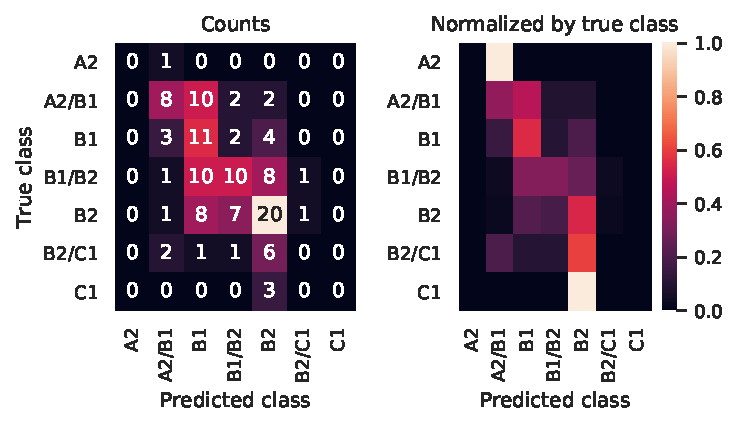
\includegraphics[width=\textwidth]{mlp-mixed-conf}
  \caption{Confusion matrix for MLP Mix}
  \label{fig:mlp-mixed-conf}
\end{figure}

\begin{figure}
  \centering
  \includegraphics[width=\textwidth]{mlp-mixed-conf-round}
  \caption{Confusion matrix for MLP Mix on collapsed labels}
  \label{fig:mlp-mixed-conf-round}
\end{figure}
